%-*- coding: UTF-8 -*-
% HYSYS_For_UTM.tex
% HYSYS_For_UTM学习
\documentclass[UTF8]{ctexart}

%添加图片
\usepackage{graphicx}

%三线表
\usepackage{booktabs}
\usepackage{tabularx}
\newcolumntype{Y}{>{\centering\arraybackslash}X}


%目录超链接
\usepackage[colorlinks,linkcolor=black]{hyperref}

%采用New Time Roman字体
\usepackage{times}
\usepackage{mathptmx}

%字体的颜色
\usepackage{color}

%段落首行缩进1格
\setlength\parindent{2em}

%设置章节标题左对齐
\CTEXsetup[format={\raggedright\bfseries\Large}]{section}
%设置章节格式
\CTEXsetup[number={\chinese{section}}]{section}
\CTEXsetup[name={第,章}]{section}


\title{HYSYS For UTM学习总结}
%author{Thomas}
\author{马青茂}
\date{\today}

\begin{document}
\maketitle

%另起一页
\newpage

\tableofcontents

%另起一页
\newpage

\section{分离塔}
% \newpage

\subsection{分离塔}
从天然气中回收液化气在天然气工业中是十分普遍的。回收主要被用来:
\begin{itemize}
	\item 生产便携的液化气
	\item 符合液化气售卖的规格
	\item 使液收最大化
\end{itemize}
HYSYS可以模拟许多不同类型、规格的精馏塔。在这个仿真中,要建立一个包含3个精馏塔的NGL厂
\begin{itemize}
	\item 脱甲烷塔
	\item 脱乙烷塔
	\item 脱丙烷塔
\end{itemize}
\textbf{学习收获:}在这章节最后,我们可以学会:
\begin{itemize}
	\item 使用Input Experts添加精馏塔
	\item 给精馏塔添加额外的设计规定
\end{itemize}
\textbf{预备知识:}在开始这个章节之前,我们需要知道如何:
\begin{itemize}
	\item 操作PFD
	\item 在PFD或WorkBook中添加物流
	\item 添加并连接单元操作
\end{itemize}
\textbf{定义仿真环境}
\begin{enumerate}	
	\item 新建一个工况
	\item 选择\textbf{Peng Robinson} EOS
	\item 添加组分:$N_2,CO_2,C_1-C_8$
	\item 进入\textbf{Simulation Environment}
\end{enumerate}
\textbf{添加进料物流}
\begin{enumerate}	
	\item 添加一股物流1,数据如下表\ref {Table1}

	\begin{table}[!htbp]
		\centering
		\caption{物流1}
		\label{Table1}
		\begin{tabularx}{\textwidth}{cY}
		\toprule
		Name & Feed1 \\
		\midrule
		Temperature & -95$^\circ$C\\
		Pressure & 2275KPa\\
		Flowrate & 1620kgmole/h\\
		Component & Mole Fraction\\
		$N_2$ & 0.0025\\
		$CO_2$ & 0.0048\\
		$C_1$ & 0.7041\\
		$C_2$ & 0.1921\\
		$C_3$ & 0.0706\\
		$i-C_4$ & 0.0112\\
		$n-C_4$ & 0.0085\\
		$i-C_5$ & 0.0036\\
		$n-C_5$ & 0.0020\\
		$C_6$ & 0.0003\\
		$C_7$ & 0.0002\\
		$C_8$ & 0.0001\\
		\bottomrule
		\end{tabularx}
	\end{table}

	\item 添加另一股物流2,数据如下表\ref{Table2}

	\begin{table}[!htbp]
	\centering
	\caption{物流2}
	\label{Table2}
		\begin{tabularx}{\textwidth}{cY}
		\toprule
		Name & Feed2 \\
		\midrule
		Temperature & -85$^\circ$C\\
		Pressure & 2290KPa\\
		Flowrate & 215kgmole/h\\
		Component & Mole Fraction\\
		$N_2$ & 0.0057\\
		$CO_2$ & 0.0029\\
		$C_1$ & 0.7227\\
		$C_2$ & 0.1176\\
		$C_3$ & 0.0750\\
		$i-C_4$ & 0.0204\\
		$n-C_4$ & 0.0197\\
		$i-C_5$ & 0.0147\\
		$n-C_5$ & 0.0102\\
		$C_6$ & 0.0037\\
		$C_7$ & 0.0047\\
		$C_8$ & 0.0027\\
		\bottomrule
		\end{tabularx}
	\end{table}
\end{enumerate}
\textbf{添加脱甲烷塔}

脱甲烷塔用Reboiled Absorber Column单元来模拟。
\begin{enumerate}
	\item 添加一股能量流,数据如下表\ref{Table3}

		\begin{table}[!htbp]
	\centering
	\caption{Ex Duty}
	\label{Table3}
		\begin{tabularx}{\textwidth}{cY}
		\toprule
		Name & Ex Duty \\
		\midrule
		Energy & $2.1\times10^6kJ/h$\\
		\bottomrule
		\end{tabularx}
	\end{table}

	\item 双击\textbf{Reboiled Absorber},进入Input Expert 界面
	\item 如下图\ref{figure1},完成输入
	\begin{figure}[!htbp]
		\centering
		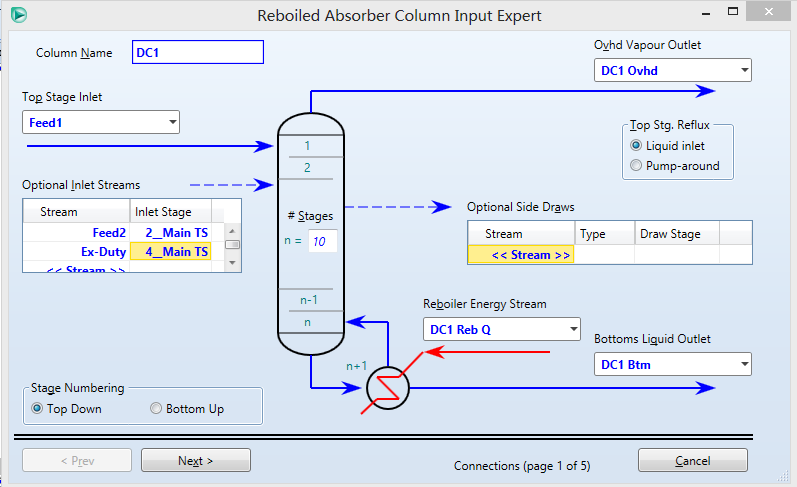
\includegraphics[scale=0.5]{DC1_Input.PNG}
		\caption{脱甲烷塔输入界面}
		\label{figure1}
	\end{figure}
	\item 点击\textbf{Next}进入下一个界面
	\item 如下图\ref{figure2},完成压力输入
	\begin{figure}[!htbp]
	\centering
	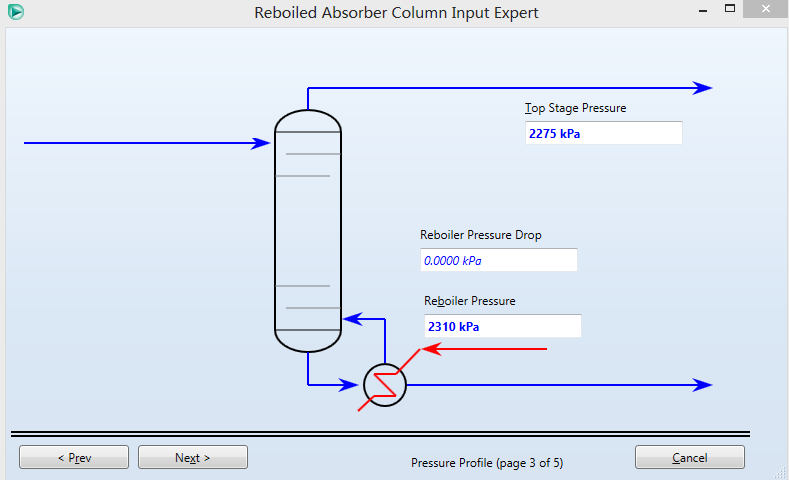
\includegraphics[scale=0.5]{DC1_Pressure.PNG}
	\caption{脱甲烷塔压力输入界面}
	\label{figure2}
	\end{figure}
	\item 点击\textbf{Next}进入下一个界面
	\item 如下图\ref{figure3},完成温度输入
	\begin{figure}[!htbp]
	\centering
	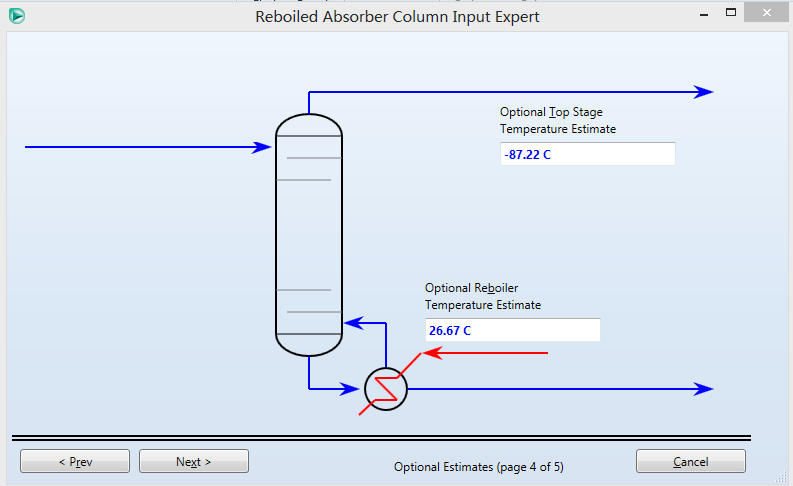
\includegraphics[scale=0.5]{DC1_Temperature.PNG}
	\caption{脱甲烷塔温度输入界面}
	\label{figure3}
	\end{figure}
	\item 点击\textbf{Next}进入下一个界面
	\item 在最后一个界面,没有信息需要输入,所以直接点击\textbf{Done}完成输入
\end{enumerate}

当点击\textbf{Done}之后,HYSYS将会打开精馏塔的参数界面,点击\textbf{Design}表格的\textbf{Monitor}页面,如下图\ref{figure4},确认塔的设计规定如图\ref{figure4}所示。你需要输入一个设计规定,塔顶产品的流率(Ovhd Prod Rate参数),设计值是$1338kgmole/h$。一旦这个值确定并输入,这个精馏塔将开始运算并应该收敛,如图\ref{figure5}
	\begin{figure}[h]
	\centering
	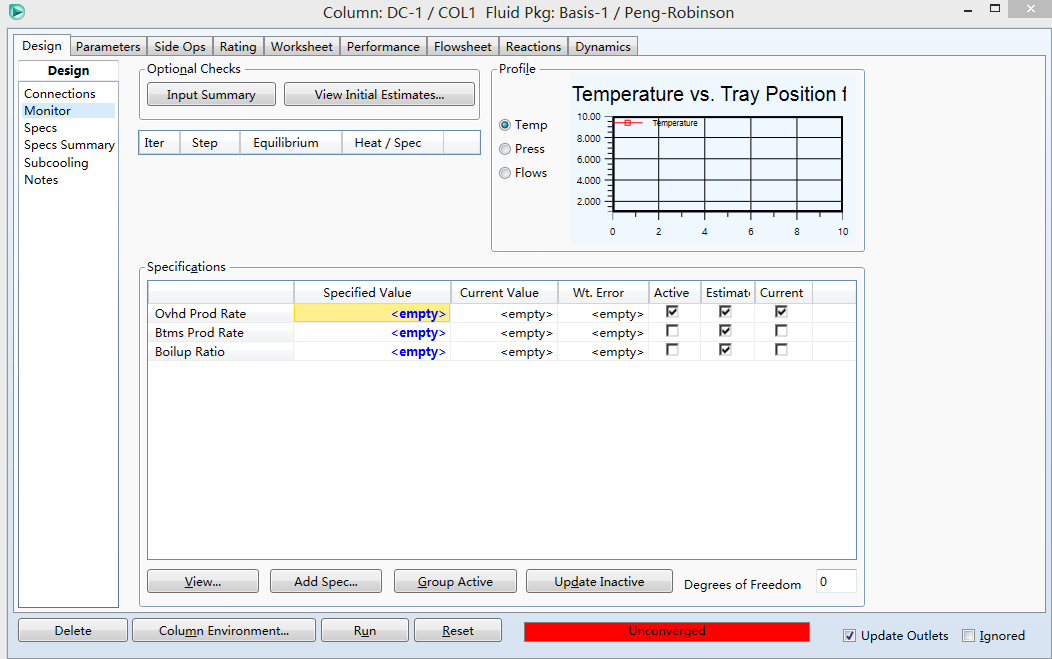
\includegraphics[scale=0.3]{DC1_Monitor.PNG}
	\caption{脱甲烷塔参数界面}
	\label{figure4}
	\end{figure}
	\begin{figure}[h]
	\centering
	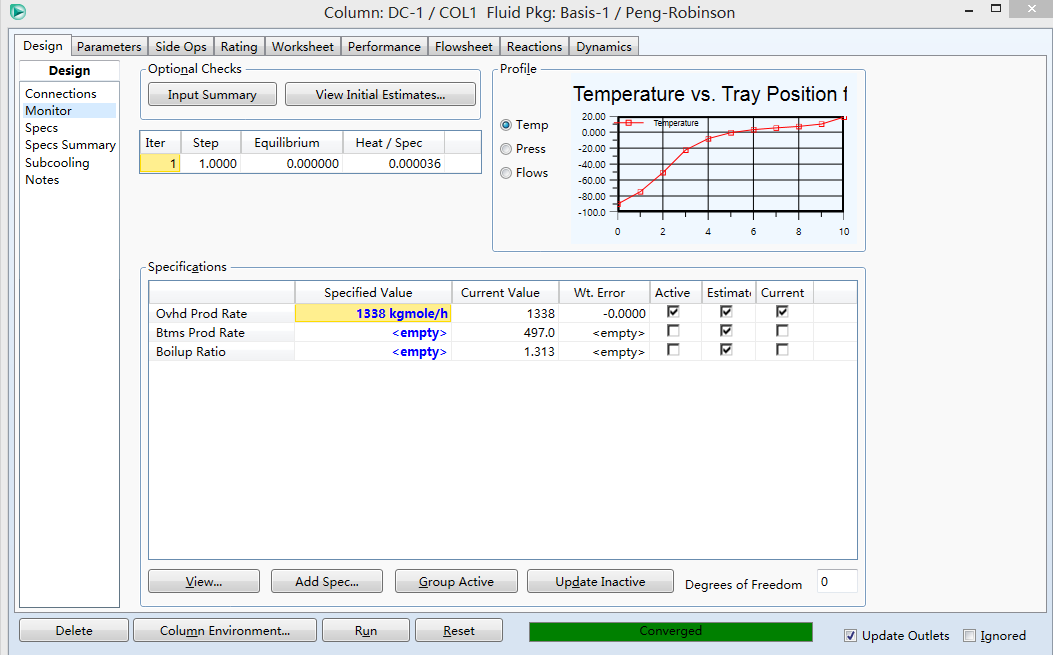
\includegraphics[scale=0.3]{DC1_Output.PNG}
	\caption{脱甲烷塔计算结果界面}
	\label{figure5}
	\end{figure}
\newpage	
\textbf{脱甲烷塔塔顶产品中的甲烷摩尔分率是多少?}\underline{$0.9686$}\\
\newline
虽然这个塔已经收敛,但塔顶流量的设计规定不总是实用的。如果塔的进料改变,那么这个设计规定会导致塔不收敛或者产品不合格。

一个可行的方法是去规定产品中任一组分的摩尔分率或者回收率。
\begin{enumerate}
	\item 进入\textbf{Design}列表中的\textbf{Specs}页面
	\item 点击\textbf{Add}创建一个新的设计规定
	\item 选中弹出列表中的\textbf{Column Component Fraction}
	\item 点击\textbf{Add Spec(s)}
	\item 按照图\ref{figure6}所示,完成设计规定
	\begin{figure}[h]
	\centering
	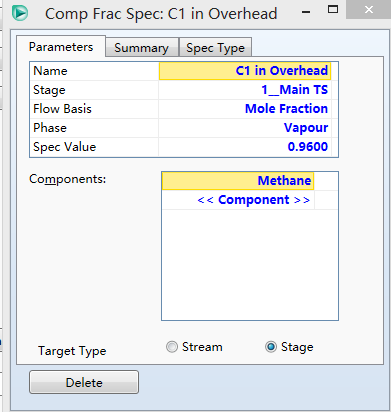
\includegraphics[scale=0.3]{DC1_Design.PNG}
	\caption{设计规定——塔顶甲烷回收率}
	\label{figure6}
	\end{figure}
	\item 关闭图\ref{figure6}中界面
	\item 进入\textbf{Monitor}页面,取消\textbf{Ovhd Prod Rate}的\textbf{Active}属性,把创建的\textbf{Comp Fraction}的\textbf{Active}属性打勾
\end{enumerate}

\textbf{脱甲烷塔塔顶产品流量是多少?}\underline{$1350kgmole/h$}
\end{document}